% !TeX root = chapter2_1d.tex
% !TeX root = thesis.tex
\ifdefined\UtilIncluded
  \renewcommand{\startchapter}[1]{}
  \renewcommand{\stopchapter}{}
  \renewcommand{\undefinedlabel}[2]{}
\else

\newcommand{\startchapter}[1]{\begin{document}\setcounter{chapter}{#1}\addtocounter{chapter}{-1}}
\newcommand{\stopchapter}{\printbibliography[title=Bibliography,heading=bibintoc]\end{document}}


\documentclass{book}
\usepackage[utf8]{inputenc}


\usepackage{geometry}
\geometry{
  papersize={170mm,240mm},
}

\usepackage{amsfonts,amsmath, amsthm, amssymb, mathtools}
\usepackage{xspace}
\usepackage[hidelinks,bookmarks,pdfusetitle]{hyperref}
\usepackage{listings}
\usepackage[pdftex]{graphicx}
\usepackage{bm}
\usepackage[english]{babel}
\usepackage{caption}
\usepackage{subcaption}
\usepackage[usenames,dvipsnames]{xcolor}
\usepackage{physics}
\usepackage{multicol}
\usepackage{xstring}
\usepackage{pythonhighlight}
\usepackage{parskip}
\usepackage{thmtools}
\usepackage{relsize}
\usepackage{bookmark}
\usepackage{lmodern}
\usepackage{ifthen}
\usepackage{biblatex}
\usepackage{microtype}
\usepackage{csquotes}
\usepackage{numprint}
\usepackage{mleftright}
\npthousandsep{{\ifmmode\mskip2mu\else\hskip0.2em\fi}}
\npdecimalsign{.}

\addbibresource{references.bib}

\newtheorem{theorem}{Theorem}[chapter]
\newtheorem{lemma}[theorem]{Lemma}
\newtheorem{corollary}[theorem]{Corollary}
\newtheorem{definition}[theorem]{Definition}

\DeclareRobustCommand{\oneD}{{1{\relsize{-1}D}}\xspace}
\DeclareRobustCommand{\twoD}{{2{\relsize{-1}D}}\xspace}
\DeclareRobustCommand{\threeD}{{3{\relsize{-1}D}}\xspace}
\DeclareRobustCommand{\cpp}{{{C\nolinebreak[4]\hspace{-.05em}\raisebox{.4ex}{\relsize{-3}\textbf{++}}}\xspace}}
\pdfstringdefDisableCommands{%
  \def\cpp{C++}%
  \def\oneD{1D}%
  \def\twoD{2D}%
  \def\threeD{3D}%
}

\newcommand{\longchapter}[2][]{%
  \chapter[#2]{#2}%
  \ifthenelse{\equal{#1}{}}{}{\chaptermark{#1}}}

\newcommand{\NN}{\mathbb{N}}
\newcommand{\ZZ}{\mathbb{Z}}
\newcommand{\QQ}{\mathbb{Q}}
\newcommand{\QQbar}{\overline{\mathbb{Q}}}
\newcommand{\RR}{\mathbb{R}}
\newcommand{\CC}{\mathbb{C}}

\newcommand{\Eigen}{\texttt{Eigen}}

\newcommand{\sage}{\texttt{sage}\xspace}

\newcommand{\hamiltonian}{\mathcal{H}}

\newcommand{\transposesign}{\intercal}
\newcommand{\transpose}[1]{{#1}^\transposesign}
\newcommand{\adjointsign}{\text{H}}
\newcommand{\adjoint}[1]{{#1}^\adjointsign}

\newcommand{\xmin}{{x_{\text{min}}}}
\newcommand{\xmax}{{x_{\text{max}}}}
\newcommand{\ymin}{{y_{\text{min}}}}
\newcommand{\ymax}{{y_{\text{max}}}}

\newcommand{\Cbottom}{\vb{C}_\text{bottom}}
\newcommand{\Ctop}{\vb{C}_\text{top}}
\newcommand{\ubottom}{\vb{u}_\text{bottom}}
\newcommand{\utop}{\vb{u}_\text{top}}

\DeclareMathOperator{\diag}{diag}
\DeclareMathOperator{\tridiag}{tridiag}
\DeclareMathOperator{\eigs}{eigs}
\DeclareMathOperator*{\argmin}{arg\,min}
\DeclareMathOperator{\Ai}{Ai}
\DeclareMathOperator{\Bi}{Bi}
\DeclareMathOperator{\OO}{\mathcal{O}}

% https://tex.stackexchange.com/a/18192/163747
\makeatletter
\newcommand{\undefinedlabel}[2]{%
  \protected@write \@auxout {}{\string \newlabel {#1}{{#2}{\thepage}{#2}{#1}{}} }%
  \hypertarget{#1}{}
}
\makeatother

\fi
\gdef\UtilIncluded{}


\startchapter{2}

\longchapter[The \oneD Schrödinger equation]{The one-dimensional time-independent Schrödinger equation}\label{cha:c2}

\section{Introduction}

The one-dimensional time-independent Schrödinger equation is an eigenvalue problem with boundary conditions. Solutions are given as an eigenvalue $\lambda \in \RR$ with corresponding eigenfunction $y: \RR \to \RR$. These eigenfunctions are defined over the bounded domain $[a, b] \subseteq \RR$ of the problem. Each solution has to satisfy the following equation
$$
    -y''(x) + V(x)y(x) = \lambda y(x)
$$
for each of the values $x\in [a, b]$. In this equation the given function $V: \RR \to \RR$ is the potential of the problem at hand. Note that in general if $y(x)$ is an eigenfunction, $c\,y(x)$ will also be an eigenfunction with the same eigenvalue, for each value of $c \in \RR$. As such, it is not really possible to say ``\emph{the} eigenfunction of corresponding to a certain eigenvalue". Later on we will prove that in many cases the eigenfunction is, up to a constant factor, uniquely defined.

Boundary conditions have to be specified before solutions can be found. These conditions pose restrictions on $y(a)$, $y'(a)$, $y(b)$ and $y'(b)$. Boundary conditions come in many flavors. We provide an overview of the most common ones:
\begin{itemize}
    \item \emph{Dirichlet boundary conditions} specify which value the solution takes on the boundary of the domain. In our case, eigenfunctions can always be scaled, as such, it is not useful to specify the value of the solution different from zero on the boundary. This type of boundary condition thus simplifies to $y(a) = 0$ and $y(b) = 0$.
    \item \emph{Neumann boundary conditions} specify which value the derivative of a solution takes on the boundary of the domain. In our case, the same remark as given for the Dirichlet boundary conditions applies. This means that Neumann boundary conditions imply that $y'(a) = 0$ and $y'(b) = 0$.
    \item \emph{Robin boundary conditions} are a generalization of both previous boundary conditions. When these conditions are imposed on a solution $y(x)$ we imply that a certain weighted average of the function and its derivative are a fixed value. As solutions can always be scaled, Robin boundary conditions can be, in our case, rewritten to
          $$
              \alpha_a y(a) + \beta_a y(a) = 0 \text{ and } \alpha_b y(b) + \beta_b y(b) = 0  \text{.}
          $$
    \item \emph{Periodic boundary conditions} are used to specify that a solution should be periodic. In other words, the solutions has to end in the same value as it started, and so should the derivative. Mathematically this can be written as: $y(a) = y(b)$ and $y'(a) = y'(b)$. These condition can be extended to \emph{anti-periodic boundary conditions}: $y(a) = -y(b)$ and $y'(a) = -y'(b)$. Or even generalized to
          $$
              \begin{pmatrix} y(a) \\ y'(a) \end{pmatrix} = \vb{K} \begin{pmatrix} y(b) \\ y'(b) \end{pmatrix}\text{.}
          $$
\end{itemize}

Note that Dirichlet or Neumann boundary conditions can always be written as Robin boundary conditions. So when studying the one-dimensional time-independent Schrödinger equation it is most general to always consider Robin boundary conditions. Periodic (or generalized periodic) boundary conditions are less common and give rise to more edge cases and subtleties. This case will be later studied in section \ref{sec:1d_periodic}.

\subsection{Properties of the Sturm-Liouville equation}

Before developing numerical methods for solving these equations it is important to build a strong theoretical foundation. The goal is to build a thorough understanding of the Schrödinger equation and use this intuition to develop efficient and accurate numerical algorithms to solve this equation.

In the scientific literature it is quite rare to find studies about the one-dimensional Schrödinger equation itself. Most, if not all, articles and books cover the more general Sturm-Liouville theory. As Sturm-Liouville equations are a generalization of Schrödinger equations they are more wildly applicable, and so more useful to study. In this section, we will follow the tradition from the literature and study the Sturm-Liouville equation. Many more details and examples of the Sturm-Liouville theory can be found in relevant textbooks, for example \cite[Chapter~5]{sagan_boundary_1961}.

The Sturm-Liouville equation is a boundary value eigenproblem, given by the following equation on the bounded domain $[a, b]$
$$
    -(p(x) y'(x))' + q(x) y(x) = E w(x) y(x)\text{.}
$$
The continuous and finite functions $p(x)$, $q(x)$ and $w(x)$ are given on the domain. These functions define the problem. A solution consists of an eigenvalue $E$ with corresponding eigenfunction $y(x)$. For now, we will study the Sturm-Liouville equation with Robin boundary conditions:
$$
    \alpha_a y(a) + \beta_a p(a) y'(a) = 0 \text{ and } \alpha_b y(b) + \beta_b p(b) y'(b) = 0\text{.}
$$

Note that the Schrödinger equation with Robin boundary conditions is a special case of the Sturm-Liouville equation. Namely, when $p(x) = 1$, $q(x) = V(x)$ and $w(x) = 1$.

    {\color{red}

        Following from the mathematical background chapter:
        \begin{itemize}
            \item Eigenvalues are real and ordered.
            \item Eigenfunctions can be orthonormal
        \end{itemize}

        In finite and non-periodic cases: eigenvalues are unique.

        \subsection{Liouville's transformation}
        Liouville provided, under certain conditions, a transformation to reduce the Sturm-Liouville equation back to the Schrödinger equation. This transformation can be used to employ the easier numerical algorithms for Schrödinger equations, to solve more general Sturm-Liouville equations.

    }



\section{Background about Matslise}

Numerical methods for ordinary differential equations as \emph{initial value} problems are already more than a century old. In particular, linear multistep methods and Runge-Kutta methods were described around 1900. First they were applied and calculated by hand, later on ``calculating machines'' \cite{milne_numerical_1926} were used. Nowadays, modern computers do all the tedious computations.

For ordinary differential equations as \emph{boundary value} problems, such as the Sturm-Liouville equations, the story is different. There still are very few general methods for such problems. For linear ordinary differential equations, one of the more popular choices is a method based upon finite differences.

\begin{figure}
    \begin{center}
        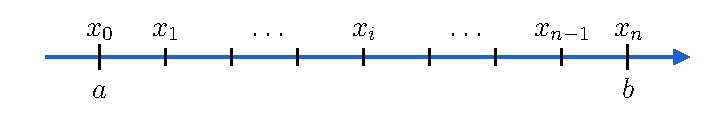
\includegraphics[width=\textwidth]{img/chapter2/finite_difference_grid.pdf}
    \end{center}
    \caption{An equidistant division of the domain $[a, b]$ in $n$ intervals.}
    \label{fig:c2_finite_difference_grid}
\end{figure}

The idea for these kinds of methods, is to discretize the integration domain $[a, b]$ into an equally spaced grid of points $a = x_0$, $x_1$, $\dots$, $x_i$, $\dots$, $x_{n-1}$, $x_{n} = b$, with $\Delta x$ the distance between two consecutive points. This discretization can be seen in figure \ref{fig:c2_finite_difference_grid}. The differential equation is now approximated by using finite difference expressions of the involved derivatives. This leads to a linear matrix-vector reformulation of the differential equation, which can be solved with classical linear algebra tools.

\subsubsection{Finite difference approximation of the Sturm-Liouville equation}

Around 1990 the best methods \cite{andrew_correction_1985,vandenberghe_accurate_1991} for approximating solutions to the Sturm-Liouville equation looked at the simpler form of the Schrödinger equation and employed a finite difference scheme. After the fact, they applied some corrections to improve the accuracy of higher eigenvalues. They experimented with which finite difference approximations to use. First they tried classical formulae, later they developed highly tuned exponential fitted formulae to better handle the oscillatory nature of the eigenfunctions.

To illustrate this class of finite difference methods for Sturm-Liouville equations we will develop a simpler version ourselves. This will allow us to appreciate the nuances of these methods more, and it will give us some ideas about the general disadvantages of this technique. The Sturm-Liouville equations we will consider are given by
\begin{equation}\label{equ:c2_finite_difference_slp}
    -(p(x)y')' + q(x) y = \lambda w(w) y\text{.}
\end{equation}
Solutions consist of eigenvalues $\lambda$ and corresponding eigenfunctions $y(x)$ such that \eqref{equ:c2_finite_difference_slp} is satisfied on the domain $[a, b]$ with homogeneous Dirichlet boundary conditions $y(a) = y(b) = 0$.

As a first step we discretize the domain $[a, b]$ with $n+1$ equidistant points, as in figure \ref{fig:c2_finite_difference_grid}. The eigenfunctions $y(x)$ we are looking for, can now be approximated by values in each of the grid points $y(x_i) \approx y_i$. For translating this problem into a linear matrix-vector equation, we are missing one key component. We still need a way to discretize the expression $(p(x) y')'$. For this, we apply the central second order finite difference formula for the first derivative twice, with half the step size. In more detail, the first derivative of a scalar function $f(x)$ can be approximated as:
$$
    f'(x) \approx \frac{f(x + h) - f(x - h)}{2h}\text{.}
$$

Applying this expression once to $(p(x) y')'$ in the point $x_i$, with step size $h = \frac{\Delta x}{2}$ gives:
$$
    (p(x) y')'(x_i) \approx \frac{1}{\Delta x}\left((p y')\left(x_{i+\frac{1}{2}}\right) - (p y')\left(x_{i-\frac{1}{2}}\right))\right)\text{.}
$$
Applying the finite difference formula a second time, with step size $\frac{\Delta x}{2}$ to approximate $y'(x)$ yields:
$$
    (p(x) y')'(x_i) \approx \frac{1}{\Delta x^2}\left(p_{i+\frac{1}{2}} y_{i+1} - \left(p_{i-\frac{1}{2}} + p_{i+\frac{1}{2}}\right) y_i + p_{i-\frac{1}{2}} y_{i-1}\right)
$$
To ease notation we have substituted $y(x_i)$ with its approximation $y_i$, and have denoted $\frac{x_i + x_{i+1}}{2}$ as $x_{i+\frac{1}{2}}$, and $p(x_i)$ as $p_i$. Also, note that if $p(x) = 1$ this formula simplifies to the classical, well-known, central second order approximation of the second derivative.

If we apply this finite difference approximation to \eqref{equ:c2_finite_difference_slp} in each point $x_i$. We get the linear generalized eigenvalue problem:
$$
    -\frac{1}{\Delta x^2}\left(p_{i+\frac{1}{2}} y_{i+1} - \left(p_{i-\frac{1}{2}} + p_{i+\frac{1}{2}}\right) y_i + p_{i-\frac{1}{2}} y_{i-1}\right) + q(x_i) y_i = \lambda w(x_i) y_i \text{.}
$$

To emphasize that this is a linear algebra problem we can rewrite this in matrix notation:
\begin{equation}\label{equ:c2_finite_difference_matrix_problem}
    \left(-\vb{D} + \diag(\vb{q})\right)\vb{y} = \lambda \diag(\vb{w}) \vb{y}\text{.}
\end{equation}

The $(n-1)$-dimensional vector $\vb{y} = \transpose{\begin{pmatrix}y_1 & y_2 & \dots & y_{n-1}\end{pmatrix}}$ is the unknown approximation of the eigenfunction. The $(n-1)$-dimensional vectors $\vb{q} = \transpose{\begin{pmatrix}q(x_1) & q(x_2) & \dots & q(x_{n-1})\end{pmatrix}}$  and $\vb{w} = \transpose{\begin{pmatrix}w(x_1) & w(x_2) & \dots & w(x_{n-1})\end{pmatrix}}$ are the values of the coefficient functions $q$ and $p$. And lastly, the matrix $\vb{D}$ is the tridiagonal matrix given by:
$$
    \vb{D} = \frac{1}{\Delta x^2}\begin{pmatrix}
        -p_{\frac{1}{2}} -p_{\frac{3}{2}} & p_{\frac{3}{2}}                   &                                   &                     &                                            \\
        p_{\frac{3}{2}}                   & -p_{\frac{3}{2}} -p_{\frac{5}{2}} & p_{\frac{5}{2}}                   &                     &                                            \\
                                          & p_{\frac{5}{2}}                   & -p_{\frac{5}{2}} -p_{\frac{7}{2}} & p_{\frac{7}{2}}     &                                            \\
                                          &                                   &                                   & \ddots              &                                            \\
                                          &                                   &                                   & p_{n - \frac{3}{2}} & -p_{n - \frac{3}{2}} - p_{n - \frac{1}{2}} \\
    \end{pmatrix}{}\text{.}
$$

To find the eigenvalues of \eqref{equ:c2_finite_difference_matrix_problem} one can notice that if $w(x_i)$ is never $0$ for $0 < i < n$ then $\diag(\vb{w})$ is invertible and the problem becomes a simple tridiagonal eigenvalue problem. This can then be solved with our favorite tridiagonal eigenvalue solver. If $w$ happens to be constant, this becomes a symmetric tridiagonal matrix, for which LAPACK \cite{lapack}, for example, contains the specialized routines: \texttt{?stev} and relatives.

\begin{figure}
    \begin{center}
        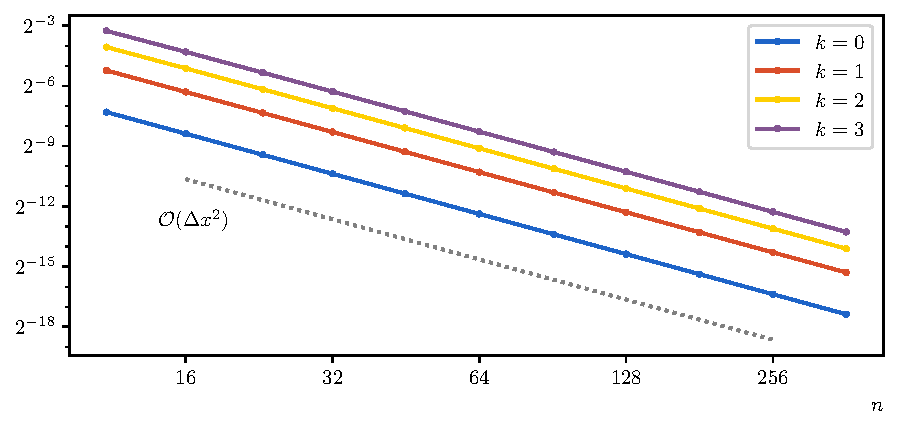
\includegraphics[width=\textwidth]{img/chapter2/finite_difference_h_error.pdf}
    \end{center}
    \caption{Relative error of approximated eigenvalues of problem \eqref{equ:c2_fd_test_problem} in function of the grid size $n$ on the domain.}
    \label{fig:c2_fd_h_error}
\end{figure}

\begin{figure}
    \begin{center}
        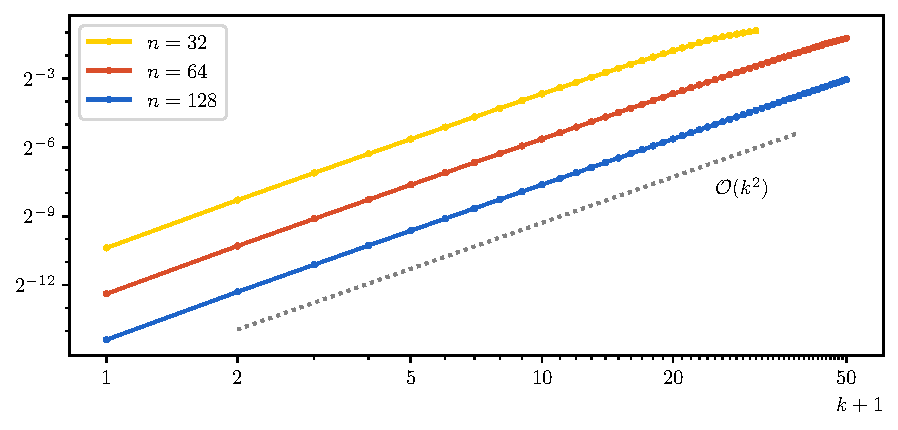
\includegraphics[width=\textwidth]{img/chapter2/finite_difference_k_error.pdf}
    \end{center}
    \caption{Relative error of approximated eigenvalues of problem \eqref{equ:c2_fd_test_problem} in function of the eigenvalue index $k$.}
    \label{fig:c2_fd_k_error}
\end{figure}

As a numerical experiment of this method we will take a look at the following Sturm-Liouville equation:
\begin{equation}\label{equ:c2_fd_test_problem}
    -\left((1+x)^2 y \right)' + (x^2 - 2) y = \lambda e^x y
\end{equation}
on the domain $[0, 1]$ with homogeneous Dirichlet boundary conditions. Figure \ref{fig:c2_fd_h_error} shows the relative errors of the 4 lowest eigenvalues in function of the chosen grid size $n$. As $n$ increases, the error decreases, as desired. Notice that as the constructed method is based upon second order finite difference formulae, we expect to see the decrease of error be of second order too, as indicated in the figure with the dotted line. This constructed method is of relatively low order, so to compute very accurate estimations, a large grid size is needed. In the literature one can find many such methods, even with much higher orders. These better methods can reach high accuracy with relatively little computational work, for the first few eigenvalues.

As earlier hinted, this type of method struggles with the computation of higher eigenvalues. Figure \ref{fig:c2_fd_k_error} illustrates this. Here, the relative error of the first 50 eigenvalues is plotted, for different values of $n$. Note that in the case of $n = 32$, only $32$ eigenvalues can be computed. On this figure, the line corresponding to $\mathcal{O}(k^2)$ is drawn. Together with the $\mathcal{O}(\Delta x^2)$ from earlier, this indicates that the relative error of the $k^\text{th}$ eigenvalue is expected to be
$$
    \mathcal{O}(\Delta x^2 k^2)
$$
for this method applied to problem \eqref{equ:c2_fd_test_problem}. This teaches us, for this method in particular, but also applies to all methods of this type, that the larger the eigenvalue, the more difficult it is to compute accurately. In the literature one can find some techniques to mitigate this effect by applying some corrections after the fact. In \cite{andrew_correction_1985} such a correction is analyzed when applied to Numerov's method. Here, the authors are able to bring the error down from $\mathcal{O}(k^6 h^4)$ to $\mathcal{O}(k^3 h^4)$. This is remarkably better. But even with this correction technique, computing large eigenvalues is still computationally difficult.

\subsection{CP-methods}

The drawbacks of the methods based upon finite differences are already known for a long time. One of the first\footnote{In \cite{ledoux_solving_2010} a brief historical overview is given of the application of CP-methods to Sturm-Liouville problems. In this thesis we will take the time to take a closer look at the earlier methods. They will provide us a more intuitive understanding of the algorithms, in preparation of our own advancements within employing these ideas.} works that tries to not only mitigate these troubles but rather fully fix them, was \cite{canosa_new_1970} in 1970. There, Canosa and De Oliveira present a new method to approximate solutions to the one dimensional time-independent Schrödinger equation. This lays the foundation to what would later be called constant perturbation methods (CPM or CP-methods). To intuitively appreciate these CP-methods it is valuable to study the method from \cite{canosa_new_1970}.

For this, we will only consider the Schrödinger equation
\begin{equation}\label{equ:c2_cpm_schrodinger}
    - y'' + V(x) y = \lambda y
\end{equation}
on the domain $[a, b]$ with homogeneous Robin boundary conditions $\alpha_a y(a) + \beta_a y(a) = 0$ and $\alpha_b y(b) + \beta_b y(b) = 0$. But do note, that using Liouville's transformation all Sturm-Liouville problems can be transformed into Schrödinger problems.

\subsubsection{Piecewise constant approximation of the potential}

\begin{figure}
    \begin{center}
        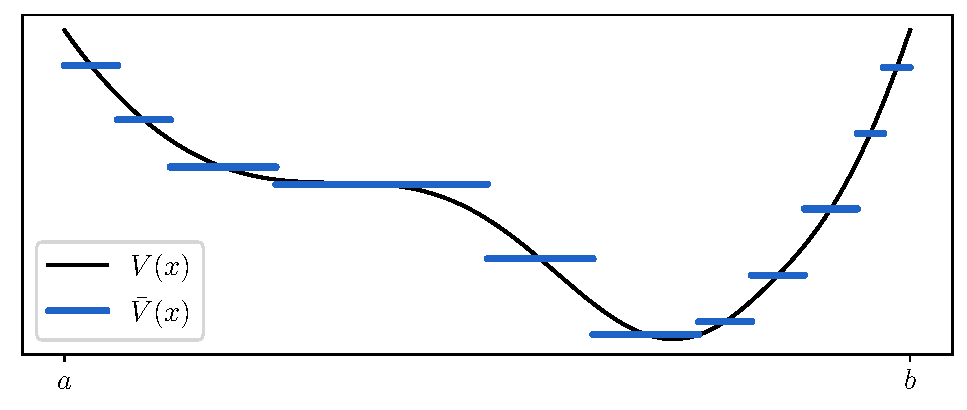
\includegraphics[width=\textwidth]{img/chapter2/cpm_constant_approx.pdf}
        \caption{A potential function $V(x)$ is approximated as the piecewise constant function $\bar{V}(x)$ along the domain $[a, b]$.}
        \label{fig:c2_cpm_constant_approx}
    \end{center}
\end{figure}

As a very first step, \cite{canosa_new_1970} simplifies the potential $V(x)$ as a piecewise constant approximation $\bar{V}(x)$. This approximation is visualized in figure \ref{fig:c2_cpm_constant_approx}. Notice that no restrictions are placed upon the size of the pieces. Upon choosing $\bar{V}(x)$, one should keep in mind that the better the piecewise approximation is, the better the resulting eigenvalues will be. And, The computational runtime depends linearly on the number of pieces.

The next step is to fixate the value for $\lambda$. Now, for each of the pieces of $\bar{V}$ the analytical solutions is computed of the problem
$$
    y'' = (V_i - \lambda) y\text{.}
$$
Here, $V_i$ is the value of $\bar{V}$ on the $i^\text{th}$ piece $[x_i, x_{i+1}]$. These analytical solutions $\psi_i(x)$ have the following structure.
$$
    \psi_i(x) = \begin{cases}
        A_i + B_i x                                                         & \text{ if $V_i = \lambda$} \\
        A_i \cos(x\sqrt{\lambda - V_i}) + B_i \sin(x\sqrt{\lambda - V_i})   & \text{ if $V_i < \lambda$} \\
        A_i \cosh(x\sqrt{V_i - \lambda}) + B_i \sinh(x\sqrt{V_i - \lambda}) & \text{ if $V_i > \lambda$}
    \end{cases}
$$

To determine the appropriate values for $A_i$ and $B_i$ continuity conditions between pieces are applied:
$$
    \psi_{i-1}(x_i) = \psi_{i}(x_i) \text{ and } \psi_{i-1}'(x_i) = \psi_{i}'(x_i) \text{.}
$$
If $n$ pieces are used, this system of equations has $2n$ variables and $2(n-1)$ equations. Together with the two equations from the boundary conditions, this yields a fully determined linear system. To find eigenvalues $\lambda$ for which an eigenfunction exists such \eqref{equ:c2_cpm_schrodinger} is satisfied, the question now becomes: for which values of $\lambda$ does the previously described system of equations has non-zero solutions? Because only these solutions correspond to a non-zero eigenfunction.

Finding values for $\lambda$ for which the constructed system becomes singular is not as trivial as one may assume. In \cite{canosa_new_1970}, the authors have provided their own root finding algorithm based upon finding changes in the sign of the determinant. But this algorithm is not without issue. Eigenvalues may be arbitrarily close together, which makes it hard to ensure you have found all requested values. Choosing the appropriate step sizes when eigenvalues become increasingly sparse is a balance between efficiency and not missing any. Later on we will describe a way to reliably and efficiently determine all required eigenvalues.

One of the main benefits of this ``new method for the solution of the Schrödinger equation'' is that its accuracy does not depend on the size of the requested eigenvalue. Because only analytical solutions of the piecewise approximated problem are considered, oscillations can be represented exactly. Even the most extreme oscillations are cleanly captured inside the $\sin$ en $\cos$ of $\psi_i$. The idea of using analytical solutions allowed the development of the CP-methods.

When building upon this method one can make an observation when looking at figure \ref{fig:c2_cpm_constant_approx}. $\bar{V}(x)$ is a crude approximation of the function $V(x)$. This remark becomes even more important when one realizes that the accuracy of the method solely depends upon the accuracy of this approximation.

The idea of Canosa and De Oliveira gained traction. In 1971 Ixaru \cite{ixaru_error_1972} has written a note about the error analysis of this new method. And in the same year Pruess \cite{pruess_estimating_1973} has studied this method thoroughly and provided numerical examples of linear piecewise approximations and quadratic piecewise approximations of the potential function. Here we will state the most important theorems, without proof. All details can be found in \cite{pruess_estimating_1973}.

\begin{theorem}[Pruess 1973]\label{the:c2_pruess_1973_1}
    Let $\lambda_k$ be the $k^\text{th}$ eigenvalue of the Schrödinger equation
    $$
        -y'' + V(x) y = \lambda y
    $$
    on the domain $[a, b]$ with homogeneous Robin boundary conditions. And let $\tilde{\lambda}_k$ be the $k^\text{th}$ eigenvalue of the approximate Schrödinger equation with potential $\bar{V}(x)$ on the same domain, with identical boundary conditions. Here $\bar{V}(x)$ is a piecewise $m^\text{th}$ degree polynomial approximation, let $h$ be the width of the largest piece in this approximation. For $h$ sufficiently small, we have as $h \to 0$,
    $$
        |\lambda_k - \tilde{\lambda}_k| = \mathcal{O}(h^{2m + 2}) \text{ for each $k$.}
    $$
\end{theorem}

This theorem provides justification for the idea of Canosa and De Oliveira. Even though a constant approximation ($m = 0$) may be crude, it still is a second order method. Furthermore, the theorem suggest that expanding this method up to higher degree piecewise polynomial approximations may be worthwhile.

In \cite{pruess_estimating_1973}, the author also studies what happens to the error on the eigenvalues if $k$ is increased. In \cite{canosa_new_1970} it was assumed that this error does not get worse as $k$ increases.

\begin{theorem}[Pruess 1973]\label{the:c2_pruess_1973_2}
    Following the notation from theorem \ref{the:c2_pruess_1973_1}, assume $\bar{V}(x)$ to be a least squares $m^\text{th}$ degree piecewise polynomial approximation of $V(x)$. This means, on each piece $[x_i, x_{i+1}]$, that $\bar{V}$ is the $m^\text{th}$ degree polynomial such the following is minimal
    $$
        \int_{x_i}^{x_{i+1}} \left(V(x) - \bar{V}(x)\right)^2 \dd x \text{.}
    $$

    Under this assumption, if $k \to \infty$, it holds for the relative error that
    $$
        \frac{\lambda_k - \tilde{\lambda}_k}{\lambda_k} = \mathcal{O}(k^{-4})\text{.}
    $$
\end{theorem}

This last theorem does not only say that the error does not become larger if $k$ increases, but the relative error even decreases rapidly when $k \to \infty$. Theorem \ref{the:c2_pruess_1973_2} highlights the main advantage this technique has in comparison to other state-of-the-art methods. Where many other methods become less and less accurate for large eigenvalues, this method becomes even more accurate.

\begin{figure}
    \begin{center}
        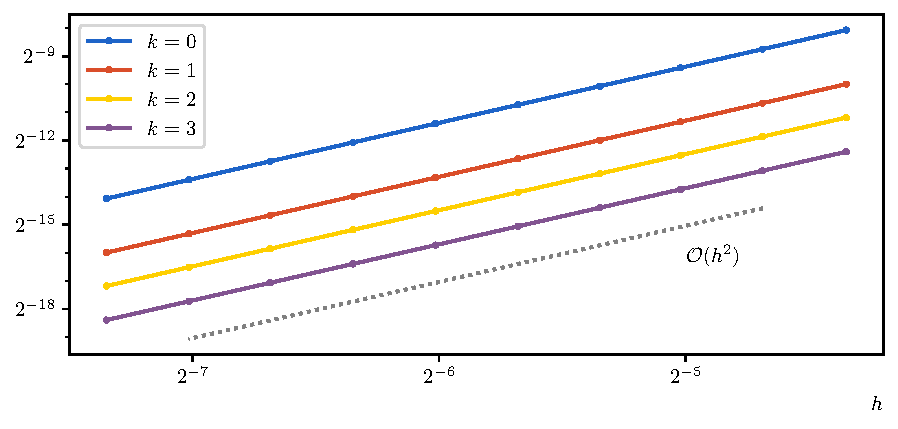
\includegraphics[width=\textwidth]{img/chapter2/pruess_h_error.pdf}
    \end{center}
    \caption{Relative error of the found eigenvalues of problem \eqref{equ:c2_pruess_test_problem} by using the method of constant piecewise approximation of the potential, with equal pieces. The graphs are in function of the size of the pieces. The most accurate calculation used $512$ pieces, the least accurate $64$.}
    \label{fig:c2_pruess_h_error}
\end{figure}

\begin{figure}
    \begin{center}
        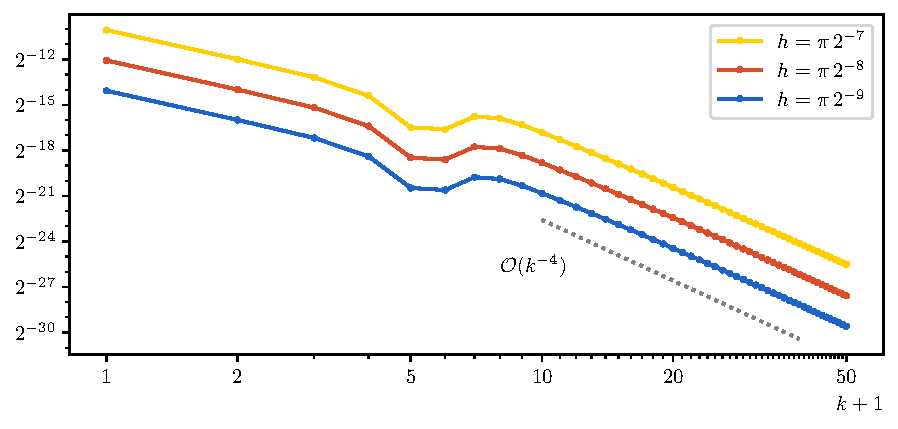
\includegraphics[width=\textwidth]{img/chapter2/pruess_k_error.pdf}
    \end{center}
    \caption{Relative error of the found eigenvalues of problem \eqref{equ:c2_pruess_test_problem} by using the method of constant piecewise approximation of the potential, with equal pieces. The graphs are in function of the index of the eigenvalue. The yellow line used $128$ pieces, the blue line $512$.}
    \label{fig:c2_pruess_k_error}
\end{figure}

As a numerical experiment we have applied the method with constant piecewise approximations ($m=0$) to the Mathieu problem
\begin{equation}\label{equ:c2_pruess_test_problem}
    -y'' + 100 \cos(x)^2 y = \lambda y
\end{equation}
on the domain $[0, \pi]$ with homogeneous Dirichlet boundary conditions. In figure \ref{fig:c2_pruess_h_error} the relative error of the application of the method is illustrated. We see that the error follows indeed the predicted line of $\mathcal{O}(h^2)$. In figure \ref{fig:c2_pruess_k_error} we see the dramatic increase in accuracy when $k$ becomes larger. The predicted order of $\mathcal{O}(k^{-4})$ seems to be reached once $k$ is sufficiently large.


But still some nuances have to be made. In \cite{pruess_estimating_1973} some numerical examples are given for constant ($m=0$), linear ($m=1$) and quadratic ($m=2$) approximations. But only for the constant approximations analytical solutions were used. For the higher order experiments, the true solution on a single piece is approximated by an at least fifteenth order Taylor series expansion. These Taylor series are only polynomial approximations of a possibly highly oscillatory function. Which, for much higher eigenvalues, gives problems.

\subsubsection{Constant perturbation methods}

In the years since the first article from Canosa and De Oliveira \cite{canosa_new_1970}, the research into these kinds of methods has flourished. One of the first extensions was to consider not only piecewise constant approximations but also linear and quadratic, as in \cite{pruess_estimating_1973}. For constant approximations, the exact solution is given by hyperbolic or trigonometric functions. For linear approximations, the Airy functions $\Ai(x)$ and $\Bi(x)$ are appropriate. As these are well-known special functions, software packages are available to evaluate them. But not unexpectedly, these packages are harder to find, and more difficult to use, than $\sin$, $\cos$ and hyperbolic variants. For quadratic, and higher order, approximations no closed form formula exists for the exact solutions.

To improve accuracy and computational efficiency, it is, when developing numerical methods, valuable to construct higher order methods. As we are limited to an order of $\mathcal{O}(h^2)$ for constant approximations, or $\mathcal{O}(h^4)$ when using linear approximations, some alternative improvements were required. In the book \cite{ixaru_numerical_1984}, Ixaru dedicated chapter 3 to the development of the constant perturbation methods. The main idea is to, not directly improve the approximation of $V(x)$. But, starting with a piecewise constant approximation $\bar{V}(x)$, adding correction terms to capture the difference between the reference solution for $\bar{V}(x)$ and the true solution for $V(x)$.

Before we deconstruct the constant perturbation methods, let us take the time to formalize which mathematical problem we are solving. For now, we will only look at the differential equation
\begin{equation}\label{equ:c2_cpm_corrected}
    y''(\delta) = (\Delta V(\delta) + \bar{V} - \lambda) y(\delta)
\end{equation}
as initial value problem starting from $0$. Denote the homogeneous Neumann solution as $u(\delta)$, as such, $u(0) = 1$ and $u'(0) = 0$. And, we will write the homogeneous Dirichlet solution as $v(\delta)$, thus $v(0) = 0$ and $v'(0)=1$. In \eqref{equ:c2_cpm_corrected}, $\bar{V}$ is a constant (not piecewise) approximation of $V(x)$ on the current piece $[x_i, x_{i+1}]$ and $\Delta V(\delta) := V(x_i + \delta) - \bar{V}$. Being able to solve the initial value problem is sufficient to also solve the boundary value eigenproblem. For solving the latter we can employ a shooting procedure to the former, see section \ref{sec:c2_shooting_prufer} for more details. The procedure we will develop here can then be applied to each of the pieces in the constant piecewise approximation of $V(x)$.

Following \cite{ixaru_numerical_1984,ixaru_cp_2000}, let us denote a solution of \eqref{equ:c2_cpm_corrected} generally as $p(\delta)$, this thus represents either $u(\delta)$ or $v(\delta)$. Now we write the solution $p(\delta)$ as a perturbation series:
$$
    p(\delta) = p_0(\delta) + p_1(\delta) + p_2(\delta) + \dots
$$
In this expression the first order term $p_0$ is the solution of the reference equation
\begin{equation}\label{equ:c2_p0_reference}
    p_0''(\delta) = (\bar{V} - \lambda) p_0(\delta)
\end{equation}
with appropriate initial values. That is, $u_0(0) = 1$ and $u_0'(0) = 0$ for $p = u$, if $p=v$ the initial values are $v_0(0)=0$ and $v_0'(0) = 1$. The perturbation corrections can now be recursively defined as the solution of
\begin{equation}\label{equ:c2_pq_definition}
    p_q''(\delta) = (\bar{V} - \lambda) p_q(\delta) + \Delta V(\delta) p_{q-1}
\end{equation}
with initial conditions $p_q(0) = p_q'(0) = 0$. Notice that this definition implies that $p$ indeed solves \eqref{equ:c2_cpm_corrected} with the appropriate initial values:
\begin{align*}
    p'' & = (\bar{V} - \lambda)p_0 + \sum_{q=1}^\infty\left((\bar{V} - \lambda)p_q + \Delta V(\delta) p_{q-1}\right) \\
        & = (\bar{V} - \lambda)\sum_{q=0}^\infty p_q + \Delta V(\delta) \sum_{q=0}^\infty p_q                        \\
        & = (\Delta V(\delta) + \bar{V} - \lambda)p\text{.}
\end{align*}

To symbolically compute the expression of $p_q$ Ixaru has introduced some auxiliary functions\footnote{What we will call $\eta_{-1}$, Ixaru has named $\xi$. The notation of the recursive definition becomes a little easier when the $\eta_m$ and $\xi$ names are unified.}, based upon the exact solution of the constant perturbation method.

\begin{definition}[Ixaru 1984]\label{def:c2_eta_functions}
    The family of $\eta$-functions $\eta_m : \RR \to \RR$ for $m \in \{-1, 0, 1, \dots\}$ is defined recursively as:
    \begin{align*}
        \eta_{-1}(Z) & = \cosh(\sqrt{Z})                                        \\
        \eta_{0}(Z)  & = \frac{\sinh(\sqrt{Z})}{\sqrt{Z}}                       \\
        \eta_{m}(Z)  & = \frac{\eta_{m-2}(Z) - (2m-1) \eta_{m-1}(Z)}{Z}\text{.}
    \end{align*}
    When $Z < 0$ the definitions of $\eta_{-1}$ and $\eta_{0}$ should be read as calculations in $\CC$. But, notice that the resulting values will always be real. Furthermore, if $Z = 0$, one should take the limit of $\eta_m$ to zero, this yields\footnote{In this expression $n!!$ is the double factorial: $n!! := n\cdot (n-2) \cdot (n - 4) \cdot ...$, with only strictly positive integers as factors. For our purposes we define $0!! = (-1)!! = 1$.} $\eta_m(0) = \frac{1}{(2m+1)!!}$.
\end{definition}

When implementing these formulas, it is more efficient to keep all calculations in $\RR$, by using $\eta_{-1}(Z) = \cos(\sqrt{-Z})$ and $\eta_{-1}(Z) = \sin(\sqrt{-Z})/\sqrt{-Z}$.

Another interesting property of these $\eta$-functions are its series expansions:\begin{align*}
    \eta_{-1}(Z) & = \sum_{q=0}^{\infty} \frac{Z^q}{(2q + 1)!}                                                      \\
    \eta_{m}(Z)  & = 2^m \sum_{q=0}^{\infty} \frac{(q+m)! Z^q}{q!(2q + 2m + 1)!} \qquad \text{if } m \geq 0\text{.}
\end{align*}
When $|Z|$ is small, the recursion from the definition becomes numerically unstable. It is more accurate to use this series expansion on $\eta_m$ and $\eta_{m+1}$, for $m$ sufficiently large, and work our way back to $m=0$ and $m=-1$ with the inverted recursion
$$
    \eta_{m-1}(Z) = Z \eta_{m+1}(Z) + (2 m + 1) \eta_{m}(Z)
    \text{.}
$$

Other interesting properties of these special functions are already studied. Here we provide some results, without proofs.
\begin{theorem}[Ixaru 1984]\label{the:c2_eta_functions}
    For the family of functions defined in definition \ref{def:c2_eta_functions}, the following properties hold for $m \in \{-1, 0, 1, 2, \dots\}$ and $Z \in \RR$.
    \begin{itemize}
        \item Asymptotic behavior for $|Z| \to \infty$:
              $$\eta_m(Z) \approx  \begin{dcases}
                      \frac{\eta_{-1}(Z)}{Z^{(m+1)/2}} & \text{if $m$ is odd}  \\
                      \frac{\eta_{0}(Z)}{Z^{m/2}}      & \text{if $m$ is even}
                  \end{dcases}$$
        \item Differentiation with respect to $Z$:
              $$
                  \eta'_{m}(Z) = \frac{1}{2}\eta_{m+1}(Z)
              $$
        \item Differentiation with respect to $\delta$ if $Z = F\delta^2$:
              \begin{align*}
                  \pdv[]{\eta_{-1}(Z)}{\delta}             & = \frac{Z}{\delta} \eta_0(Z)                           \\
                  \pdv[]{\delta^{2m+1}\eta_{m}(Z)}{\delta} & = \delta^{2m} \eta_{m-1}(Z) \qquad \text{if } m \geq 0 \\
              \end{align*}
    \end{itemize}
\end{theorem}

With the theory about the family of $\eta$-functions in hand, we are able to solve equations \eqref{equ:c2_p0_reference} and \eqref{equ:c2_pq_definition} symbolically. The following theorem from \cite{ixaru_numerical_1984} captures these symbolic calculations for $p_q(\delta)$. As these formulae have been instrumental to our work (especially for section \ref{sec:c2_cp_in_delta}), we will provide a proof.

\begin{theorem}[Ixaru 1984]\label{the:c2_perturbation_terms}
    Let $p(\delta)$ be a general solution of
    $$
        p''(\delta) = \left(\Delta V(\delta) + \bar{V} - \lambda\right)p(\delta)
    $$
    over the interval $[0, h]$. In this expression $V = \bar{V} + \Delta V(\delta)$ is a given potential function, with $\bar{V}$ a constant approximation and $\Delta V(\delta)$ the residual term. The value $\lambda$ is fixed. We denote the solution with initial conditions $u(0) = 1$ and $u'(0)=0$ as $u(\delta) = p(\delta)$, and the solution with initial conditions $v(0) = 0$ and $v'(0) = 1$ will be denoted with $v(\delta) = p(\delta)$. For ease of notation we will write $Z(\delta) = \left(\bar{V} - \lambda\right)\delta^2$. Let $p(\delta) = p_0(\delta) + p_1(\delta) + p_2(\delta) + \dots$ with:
    \begin{align*}
        p_0''(\delta) & = (\bar{V} - \lambda) p_0(\delta)                                                             \\
        p_q''(\delta) & = (\bar{V} - \lambda) p_q(\delta) + \Delta V(\delta) p_{q-1}(\delta) \quad\text{for $q > 0$.}
    \end{align*}
    The function $p_0$ inherits the initial conditions of $p$. If $q > 0$, $p_q$ has as initial conditions $p_q(0) = p_q'(0) = 0$.


    If $\Delta V(\delta)$ is a polynomial in $\delta$ then each term \(p_q\) is given by:
    \begin{align}
        p_q(\delta)  & = \sum_{i=-1}^\infty \delta^{2i+1} C^{(q)}_i(\delta) \eta_{i}(Z(\delta))  \label{equ:c2_cp_coeff_pq_formula}                                             &
        \intertext{with derivative:}
        p_q'(\delta) & = \frac{C_{-1}^{(q)}(\delta)}{\delta^2}\left(\eta_{-1}(Z(\delta))+Z(\delta)\eta_{0}(Z(\delta))\right)            \label{equ:c2_cp_coeff_pq_diff_formula}   \\\nonumber
                     & \qquad + \sum_{i=-1}^\infty \left(C_{i}^{(q)\prime}(\delta) + \delta C_{i+1}^{(q)}(\delta)\right) \delta^{2i + 1}\eta_{i}(Z(\delta)) \text{.}
    \end{align}
    The functions $ C^{(q)}_i (\delta) $ are polynomials and satisfy the following recursive relation: \begin{align*}
        C_i^{(q)}(\delta)    & = \frac{\delta^{-i}}{2} \int_0^\delta \varepsilon^{i-1} \left(
        C_{i-1}^{(q-1)}(\varepsilon) \Delta V(\varepsilon) - C_{i-1}^{(q)\prime\prime}(\varepsilon)
        \right)\dd\varepsilon                                                                 \\
        C_{i}^{(0)}(\delta)  & = \begin{cases}
            \delta & \text{if $p = u$ and $i = -1$} \\
            1      & \text{if $p = v$ and $i = 0$}  \\
            0      & \text{otherwise}
        \end{cases}                                   \\
        C_{-1}^{(q)}(\delta) & = 0 \quad \text{if $q > 0$}\,.                                 \\
    \end{align*}
\end{theorem}
\begin{proof}
As these formulae are recursively defined, a proof by induction is most natural. For $q=0$ the exact solutions can be calculated. If $\bar{V} \geq \lambda$, then $u_0(\delta) = \cosh(\sqrt{Z(\delta)})$ and $v_0(\delta) = \sinh(\sqrt{Z(\delta)})/\sqrt{\bar{V} - \lambda}$. If $\bar{V} < \lambda$ on the other hand, then $u_0(\delta) = \cosh(\sqrt{-Z(\delta)})$ and $v_0(\delta) = \sinh(\sqrt{-Z(\delta)})/\sqrt{\lambda - \bar{V}}$. By using the $\eta$-functions both these can be summarized as:
$$ u_0 = \eta_{-1}(Z(\delta)) \text{ and } v_0 = \delta\eta_{0}(Z(\delta))\text{.}$$
Substituting, for $q=0$, the values of $C^{(0)}_i$ into \eqref{equ:c2_cp_coeff_pq_formula} yields exactly the same expressions. This proves the induction basis.

Assume, as induction hypothesis, that the theorem holds for any value for $q$ less than $Q$. First we prove that for each $i$, $C_i^{(Q)}$ is a polynomial. For this we apply induction with respect to $i$. For $i = -1$, the $C^{(Q)}_{-1} =0$ is a polynomial. Because $\Delta V(\delta)$ is assumed to be polynomial, we notice that for any other $i$
$$
    C_{i-1}^{(Q-1)}(\varepsilon) \Delta V(\varepsilon) - C_{i-1}^{(Q)\prime\prime}(\varepsilon)
$$
is a polynomial, as a consequence of the induction hypothesis in $Q$, and the induction hypothesis in $i$. This implies that the integrand in the definition of $C_i^{(Q)}(\delta)$ is polynomial no terms of degree less than $i-1$. This means that the integral in that definition will be divisible by $\delta^i$. Which proves that all $C_{i}^{(Q)}$ are polynomials.

Next we proof that $p_Q(\delta)$ is a solution of
$$
    p_Q''(\delta)  = (\bar{V} - \lambda) p_Q(\delta) + \Delta V(\delta) p_{Q-1}(\delta)
$$
with initial conditions $p_Q(0) = p_Q'(0) = 0$. That $p_Q(0) = 0$ can be seen in \eqref{equ:c2_cp_coeff_pq_formula}, using the facts that $C^{(Q)}_{-1} = 0$ for $Q > 0$ and that $C_i^{(Q)}$ are polynomials. Using the properties from theorem \ref{the:c2_eta_functions}, we can compute $p_Q'(\delta)$ to be as in \eqref{equ:c2_cp_coeff_pq_diff_formula}. That this expression is zero for $\delta = 0$ is less apparent. First, notice that most terms are zero because $C_i^{(Q)}$ are polynomials and $C^{(Q)}_{-1} = 0$ for $Q > 0$. The only term for which this is not clear is with $i = -1$: $C_0^{(Q)}(0)\eta_{0}(Z(0))$. For this term, we remark that the polynomial $C^{(q)}_{-1}(\delta)$ never contains a constant term, for most values of $q$ it is zero, and for $q=0$ it can only be zero or $\delta$. This means, by the recursive construction, that $C_{i}^{(q)}(\delta)$ also does not contain a constant term. Which means $C_{i}^{(q)}(0) = 0$, and thus $p_Q'(0) = 0$, for $Q > 0$. The last thing, we still have to proof, is that this $p_Q$ indeed solves its defining equation.

For this, we compute $p_Q''$. For the sake of brevity, we will omit the argument $\delta$ from most functions, and remember that all derivatives are with respect to $\delta$. But first, we know, from the definition of $C_i^q$ that
$$
    C_i^{(q)\prime} = -i \delta^{-1} C_i^{(q)} + \frac{\delta^{-1}}{2}\left(C^{(q-1)}_{i-1}\Delta V - C^{(q)\prime\prime}_{i-1}\right)\text{,}
$$
but also that
\begin{align*}
    {\dv[]{\delta^{2i+1}\eta_i(Z)}{\delta}}               & = \delta^{2i} \eta_{i-1}                                         \\
    \text{ and } {\dv[2]{\delta^{2i+1}\eta_i(Z)}{\delta}} & = \delta^{2i-1}\left(2i\eta_{i-1}(Z) + Z\eta_i(Z)\right)\text{.}
\end{align*}

\begingroup
\allowdisplaybreaks
These expressions, together with $C_{-1}^{(Q)} = 0$, now can be used to simplify $p_Q''$:
\begin{align*}
    p_Q   & = \sum_{i=0}^{+\infty} C_{i}^{(Q)} \delta^{2i + 1} \eta_{i}(Z)                                                                            \\
    p_Q'' & = \sum_{i=0}^{+\infty} C_i^{(Q)}\delta^{2i-1}\left(2i\eta_{i-1}(Z) + Z\eta_i(Z)\right)                                                    \\
          & + \sum_{i=-1}^{+\infty} 2C_{i+1}^{(Q)\prime}\delta^{2i+2}\eta_{i}(Z) + \sum_{i=0}^{+\infty} C_i^{(Q)\prime\prime}\delta^{2i+1}\eta_{i}(Z) \\
          & = \sum_{i=0}^{+\infty} C_i^{(Q)}\delta^{2i-1}\left(2i\eta_{i-1}(Z) + Z\eta_i(Z)\right)                                                    \\
          & + \sum_{i=-1}^{+\infty} -2(i+1)C_{i+1}^{(Q)}\delta^{2i+1}\eta_{i}(Z) + p_{Q-1} \Delta V                                                   \\
          & = \frac{Z}{\delta^2}p_Q + p_{Q-1} \Delta V \text{.}
\end{align*}
\endgroup
Due to the definition of $Z = \delta^2(\bar{V} - \lambda)$, this expresses exactly that $p_Q$ is a solution to $p_Q'' = (\bar{V} - \lambda)p_Q + \delta V p_{Q-1}$. Which, in turn, proves the induction step.
\end{proof}

At first glance, it may not be clear why theorem \ref{the:c2_perturbation_terms} is that important. Still, these rather tedious computations and relatively complicated recursive relation allows us to construct formulae of any order. To calculate such a formula choose values $N$ and $Q$ and compute the values of $C_{i}^{(q)}$ for $q \leq Q$ and $i \leq N$. If $\Delta V$ is assumed to be a polynomial in $\delta$, then $C_{i}^{(q)}$ will be as well. The solution $p(\delta)$ will now take the following form:
$$
    p(\delta) = \sum_{q=0}^{Q} p_q(\delta) \text{ with } p_q(\delta) = \sum_{i=-1}^{N} C_{i}^{(q)}(\delta) \delta^{2i+1} \eta_i(Z) \text{.}
$$

{\color{red} To do: in practice, this is not sufficient. As $C$ very much depends on $V$.}

    {\color{red} To do: Some history and details about implementing these?}

\subsection{Shooting with Prüfer's transformation}\label{sec:c2_shooting_prufer}

\section{Matslise 3.0}

\cite{baeyens_fast_2020}

\subsection{CP-methods in function of \texorpdfstring{$\delta$}{delta}}\label{sec:c2_cp_in_delta}

\subsection{Architecture of the \texorpdfstring{\cpp}{C++} library}

\section{Periodic \texorpdfstring{\oneD}{1D} time-independent Schrödinger equation}
\label{sec:1d_periodic}

\begin{theorem}

\end{theorem}
\cite{binding_prufer_2012}

\stopchapter
